\chapter{Warcaby}
\thispagestyle{chapterBeginStyle}
\label{rozdzial1}

% {\color{dgray}
% Niniejszy rozdział poświęcony będzie zaznajomieniu Czytelnika z grą w Warcaby oraz szczególną wersją tej gry. Omówione również zostaną powody skupienia się nad tym wariantem, jak i inne badania przeprowadzone w przeszłości przez naukowców.
% }

% Warcaby są jedną z najpopularniejszych klasycznych gier dwuosobowych. Jest to przedstawiciel gier o doskonałej informacji, tj. gracze na każdym stadium gry posiadają pełną wiedzę na temat sytuacji na planszy oraz historii ruchów. Zaliczają się też do gier o sumie zerowej, czyli takich w których zysk jednego gracza przekłada się bezpośrednio na stratę drugiego, a zwycięzca może być tylko jeden. \ldots

Warcaby to jedna z najpopularniejszych klasycznych gier dwuosobowych, zaliczanych do gier z doskonałą informacją i gier o sumie zerowej. Przyjmuje się, że gra ta zrodziła się w XII wieku, najprawdopodobniej na południu Francji lub w Hiszpanii, oraz że wywodzi się ona z dawnej arabskiej gry Alquerque~\cite{Gry}. Istnieją coroczne turnieje i mistrzostwa światowe w różnych odmianach Warcabów, choć dzięki nieskomplikowanym zasadom są one popularne również w mniejszych kręgach.

\section{Reguły warcabów standardowych}

Pojedynczą partię Warcabów rozgrywa się na szachownicy 8x8 o polach na zmianę pomalowanych na jasno lub ciemno. W grze wykorzystywane są dwa rodzaje figur - piony i damki. Obydwaj gracze rozstawiają po 12 pionów na ciemnych polach w swoich pierwszych trzech rzędach. Dla rozróżnienia, piony pierwszego gracza są koloru białego, natomiast piony drugiego gracza - czarnego. Celem gry jest wyeliminowanie wszystkich figur przeciwnika lub zablokowanie go, poprzez serię naprzemiennych ruchów swoimi figurami. (Zablokowanie gracza oznacza doprowadzenie do takiej sytuacji, w której gracz ten nie jest w stanie wykonać żadnego legalnego ruchu w momencie gdy następuje jego kolej.)

\FloatBarrier

% \hspace{5cm}

\begin{figure}[h!]
\centering
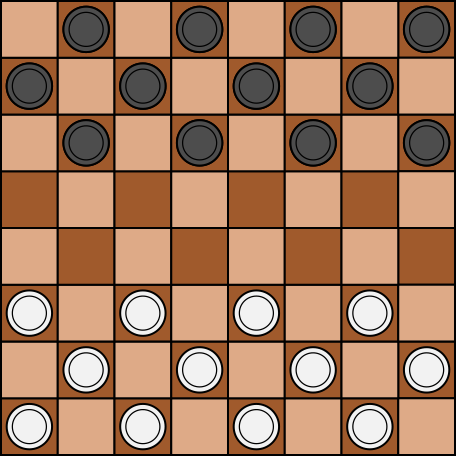
\includegraphics[scale=.6]{graphics/warcaby_planszaStartowa.png}
\caption{Stan początkowy planszy w Warcabach.}
\label{fig:plansza}
\end{figure}

\FloatBarrier

Wszystkie figury w grze mogą poruszać się tylko i wyłącznie na ukos (przez co żadne jasne pole na planszy nie zostanie zajęte przez żadną figurę w trakcie rozgrywki). Piony z którymi zaczynają gracze poruszają się tylko o jedno pole w przód względem ich właściciela. Tzn. pion może skoczyć na pole ukośnie sąsiadujące w kierunku oponenta, o ile pole to nie jest zajęte przez inną figurę. W grze istnieje również druga figura - jeżeli pion gracza dojdzie do końca planszy znajdującego się po stronie jego oponenta (do tzw. rzędu awansu), pion zamieniany jest na damkę. Damka jest najpotężniejszą figurą w grze, jako że potrafi poruszyć się we wszystkich czterech kierunkach na ukos, a na dodatek przebyć dowolną liczbę pól w linii w jednym ruchu. Pod tym względem damkę najłatwiej porównać z figurą gońca w szachach.

Każdą figurę w Warcabach można zbijać, tj. usuwać z obecnej rozgrywki. Piony mogą zbijać sąsiednie figury przeciwnika, wykonując skok nad tą figurą na następne pole w linii prostej, o ile takie pole jest wolne. Piony mogą bić zarówno do przodu, jak i do tyłu. Damki w standardowych Warcabach zbijają ze znacznie większego dystansu (można powiedzieć, że w momencie zbijania ich "sąsiadowanie" z przeciwnymi figurami nie jest ograniczone do jednego pola różnicy). Zbita figura zostaje zdjęta z planszy i nie bierze udziału w rozgrywce do momentu jej zakończenia. Nie można bić swoich figur.

Bicia w Warcabach mają specjalne reguły wyróżniające je spośród innych gier planszowych. Po pierwsze, w jednym ruchu jedna figura może wykonać wiele bić. Jeśli po jednym biciu figura wskoczyła w miejsce z którego jest w stanie przeprowadzić kolejne bicie, można takie bicie wykonać w tej samej turze. W jednym ruchu nie można dwa razy zbić tej samej figury. Po drugie, bicia są obowiązkowe. Jeżeli gracz w swojej turze jest postawiony w sytuacji w której co najmniej jedna z jego figur ma możliwość bicia, gracz ten musi wykonać taki ruch. Dodatkowo, o ile ruch bicia pionem można wybrać w przypadku większej liczby możliwych bić, damki mają obowiązek maksymalnego bicia, tj. należy przeprowadzić bicie o największej możliwej liczbie zbijanych figur w jednym ruchu.

\section{Wariant angielski}

\FloatBarrier

Praca skupiona jest na szczególnej wersji gry w Warcaby, nazywanej na ogół wariantem angielskim, lub w niektórych kręgach wariantem amerykańskim. Został on wybrany głównie ze względu na ograniczenie przestrzeni stanów w jakich może znaleźć się rozgrywka - reguły gry dostosowane do tego wariantu znacznie zmniejszają liczbę możliwości które rozgrywający algorytm musi rozpatrzeć.

% \subsection{Zmiany w zasadach}

Wariant ten wprowadza dwie zmiany do zasad gry względem wariantu standardowego (opierając się o~\cite{Gry}). Po pierwsze, zwykłe piony nie mogą bić do tyłu. Po drugie, damkom ogranicza się możliwość ruchu o dowolną liczbę pól do jednego sąsiedniego pola oraz do bicia wyłącznie sąsiadujących przeciwnych figur, lecz wciąż mogą poruszać się we wszystkich kierunkach na ukos. Jedyną przewagą damek nad pionkami w tym wariancie jest możliwość ruchu i bicia do tyłu.

% \begin{figure}
% \centering
% \begin{minipage}{.5\textwidth}
%     \centering
%     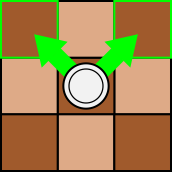
\includegraphics[scale=.6]{graphics/warcaby_ruchyPionZwykle.png}
%     \captionof{figure}{Ruchy piona w wariancie angielskim}
%     \label{fig:sub1}
% \end{minipage}%
% \begin{minipage}{.5\textwidth}
%     \centering
%     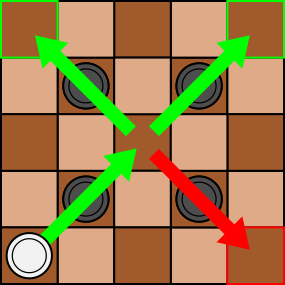
\includegraphics[scale=.6]{graphics/warcaby_ruchyPionBicia.png}
%     \captionof{figure}{Bicia piona w wariancie angielskim}
%     \label{fig:sub2}
% \end{minipage}
% \end{figure}

% \begin{figure}
% \centering
% \begin{minipage}{.5\textwidth}
%     \centering
%     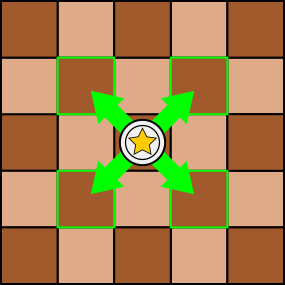
\includegraphics[scale=.6]{graphics/warcaby_ruchyDamkaZwykle.png}
%     \captionof{figure}{Ruchy damki w wariancie angielskim}
%     \label{fig:sub1}
% \end{minipage}%
% \begin{minipage}{.5\textwidth}
%     \centering
%     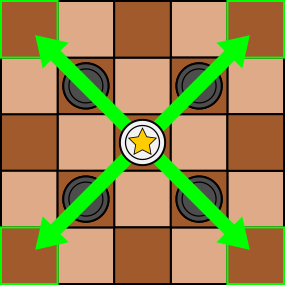
\includegraphics[scale=.6]{graphics/warcaby_ruchyDamkaBicia.png}
%     \captionof{figure}{Bicia damki w wariancie angielskim}
%     \label{fig:sub2}
% \end{minipage}
% \end{figure}

\begin{figure}
\centering
\begin{subfigure}{.5\textwidth}
  \centering
  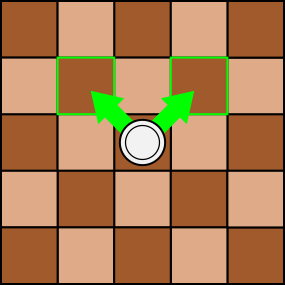
\includegraphics[scale=.6]{graphics/warcaby_ruchyPionZwykle3.png}
  \caption{Legalne ruchy}
  \label{fig:sub1}
\end{subfigure}%
\begin{subfigure}{.5\textwidth}
  \centering
  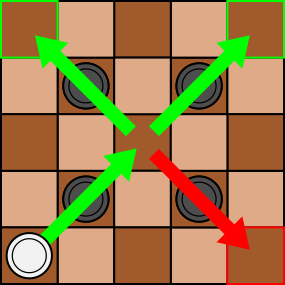
\includegraphics[scale=.6]{graphics/warcaby_ruchyPionBicia.png}
  \caption{Legalne bicia}
  \label{fig:sub2}
\end{subfigure}
\caption{Zestaw możliwych ruchów dla piona w wariancie angielskim}
\label{fig:test}
\end{figure}

\begin{figure}
\centering
\begin{subfigure}{.5\textwidth}
  \centering
  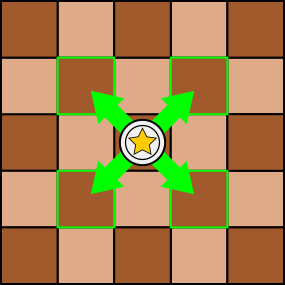
\includegraphics[scale=.6]{graphics/warcaby_ruchyDamkaZwykle.png}
  \caption{Legalne ruchy}
  \label{fig:sub11}
\end{subfigure}%
\begin{subfigure}{.5\textwidth}
  \centering
  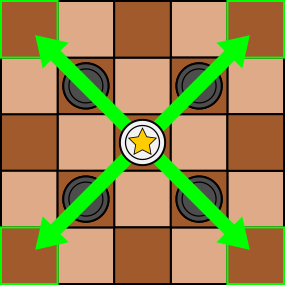
\includegraphics[scale=.6]{graphics/warcaby_ruchyDamkaBicia.png}
  \caption{Legalne bicia}
  \label{fig:sub22}
\end{subfigure}
\caption{Zestaw możliwych ruchów dla damki w wariancie angielskim}
\label{fig:test}
\end{figure}

\FloatBarrier

Przydatna w implementacji rzecz o której warto wspomnieć jest rozpatrywanie remisów. W grach towarzyskich remis zazwyczaj następuje za obopólną zgodą graczy. Na arenie turniejowej istnieje parę kryteriów determinujących remis. W rozpatrywanej wersji wariantu angielskiego wykorzystywana będzie zasada 40 ruchów, która mówi że rozgrywka kończy się remisem w momencie gdy w 40 naprzemiennych ruchach obu graczy nie została zbita ani jedna figura.

\FloatBarrier

\subsection{Badania wariantu}

Do rozwoju badań nad Warcabami w wariancie angielskim najmocniej przyczynił się Jonathan Schaeffer, profesor Uniwersytetu Alberty w Kanadzie. Jego zespół opracował Chinook'a, przeszukujący w głąb program do grania w Warcaby angielskie, który w roku 1992 oraz 1994 stanął naprzeciw ówczesnego mistrza świata Marion'a Tinsley'a i ogłoszony został pierwszym komputerowym zwycięzcą mistrzostw~\cite{Chinook}. Następnie, z pomocą programu, udowodnili poprzez słabe rozwiązanie (\textit{weakly solved}, pojęcie omówione w~\cite{Solving}) że każda gra w Warcabach angielskich kończy się remisem, pod warunkiem że gracze wykonują ruchy doskonale~\cite{Solved}. Pomimo uproszczonych zasad względem klasycznej wersji, wariant angielski posiada przestrzeń stanów wielkości rzędu $10^{20}$, dlatego też rozwiązanie zajęło zespołowi Schaeffer'a około 18 lat i 200 równolegle liczących maszyn.



